\chapter{Storia ed evoluzione dei motori scacchistici} %\label{1cap:spinta_laterale}
% [titolo ridotto se non ci dovesse stare] {titolo completo}
%
\begin{citazione}
    Questo capitolo illustra lo stato dell'arte e i lavori presenti in letteratura sugli aspetti di ricerca trattati nel nostro studio. 
    Prima di dare un'occhiata alla varietà degli approcci adottati per affrontare il problema della complessità degli scacchi, 
    è opportuno fare un passo indietro per capire meglio di \textit{che cosa} si parla.
\end{citazione}

\section{Teoria dei giochi}
La \textbf{teoria dei giochi} è una disciplina che studia gli ambienti di interazione strategica tra
agenti intelligenti\footnote{Viene definito agente un sistema in grado di percepire il suo ambiente e di agire su di esso. La peculiarità
di un agente intelligente è da ricercare nei risultati delle sue azioni che, a un osservatore comune, sembrerebbero essere prerogativa
dell'intelligenza di un essere umano.}. Per approcciare un problema di questo tipo, l'agente è necessariamente tenuto a trovare
una strategia che tenga in considerazione le possibili azioni dell'avversario. In questo contesto, una strategia specifica si considera
\textbf{ottima} se porta ad un risultato almeno pari a quello di qualsiasi altra strategia; il problema da risolvere è dunque 
quello di capire \textit{come} poter trovare una strategia ottima. Inseriti in questo contesto,
gli scacchi vengono classificati come gioco a \textbf{somma zero} (il risultato finale di un partecipante
è bilanciato dal risultato di un altro partecipante di valore uguale ma di segno opposto) e con \textbf{informazione perfetta} (gli stati
del gioco sono sempre espliciti agli agenti).
%citare

\section{Come si gioca a scacchi}
\subsection{Preparazione della scacchiera}
Le regole ufficiali del gioco degli scacchi\cite{lawsofchess} prevedono che la scacchiera sia inizialmente disposta in modo che ogni giocatore abbia una casella chiara nell'angolo inferiore destro. Ai due angoli opposti sono collocate le due torri, seguite dai due cavalli e dai due alfieri. La regina occupa sempre la casella del proprio colore, e il re è collocato accanto alla regina. Tutta la seconda traversa è invece occupata dai pedoni.
\begin{figure}[!htb]
    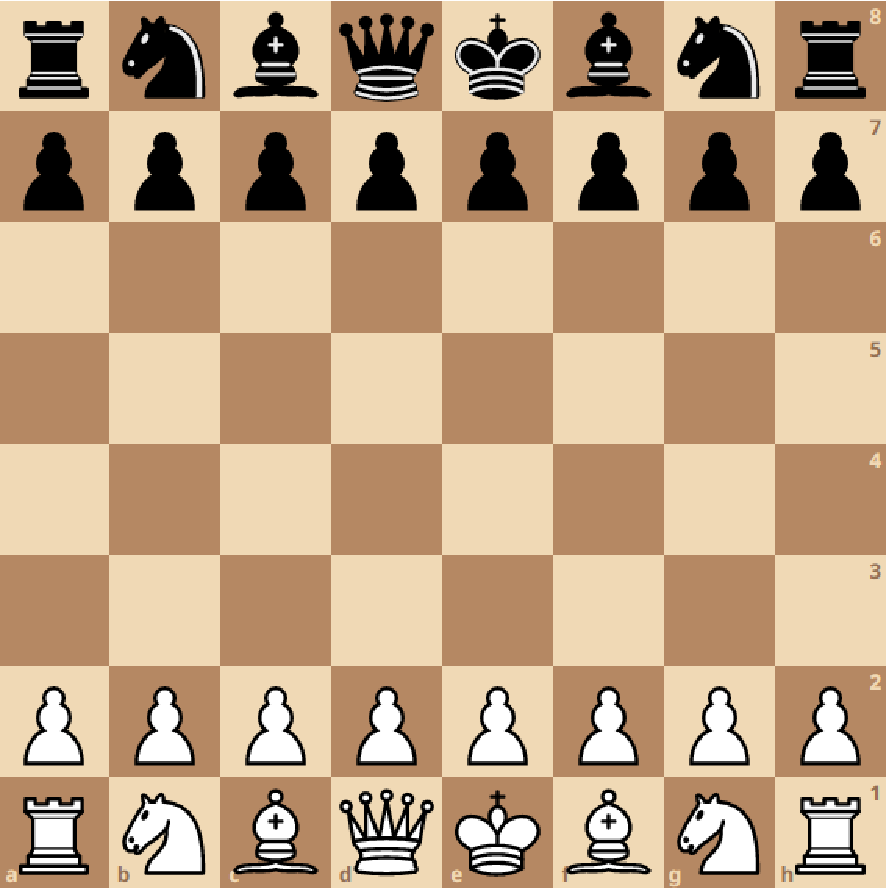
\includegraphics[width=10cm]{frontmatter/figure/scacchiera_iniziale.pdf}
    \centering
    \caption{Disposizione dei pezzi all'inizio della partita}
    \label{fig:checkmate}
\end{figure}
\subsection{Come si muovono i pezzi}
Ogni tipologia di pezzo segue delle regole ben precise nei movimenti. Non è possibile, ad esempio, muovere dei pezzi attraversando altri pezzi (eccetto per il cavallo, che può "saltarli") e ogni casella può essere occupata soltanto da un pezzo per volta. Negli scacchi è possibile liberare una casella dall'occupazione avversaria, \textbf{catturando} il pezzo interessato ed eliminandolo dalla scacchiera fino alla fine della partita. Come accennato in precedenza, ogni pezzo si muove in modo diverso dall'altro. In particolare:
\begin{itemize}
    \item il \textbf{re} può muoversi soltanto di una casella per volta nelle 8 direzioni disponibili, ma non è possibile spostarlo in una casella che lo metterebbe sotto \textbf{scacco} (minacciato da un pezzo avversario);
    \item la \textbf{regina} può muoversi in qualsiasi direzione seguendo una linea retta sia in orizzontale che in diagonale di quante caselle vuole. Come tutti gli altri pezzi, in caso di cattura di un pezzo avversario il suo movimento si conclude nella casa precedentemente occupata dal pezzo catturato;
    \item la \textbf{torre} può muoversi di quante caselle si desidera, ma soltanto in avanti, indietro e di lato. Le due torri, quando ben collegate, si proteggono a vicenda e risultano estremamente utili;
    \item l'\textbf{alfiere} può muoversi in diagonale, e in virtù di questa caratteristica ogni alfiere rimane sullo stesso colore fino alla fine della partita (uno sulle caselle chiare e l'altro sulle caselle scure);
    \item il \textbf{cavallo} segue dei movimenti "a L", avanzando di due caselle in una direzione e poi di un'altra casella a 90°;
    \item il \textbf{pedone} può muoversi di una sola casella in avanti (oppure anche due se è la sua prima mossa), ma cattura i pezzi avversari in diagonale di una casella. Non è possibile indietreggiare, né catturare all'indietro. Inoltre, se un pedone raggiunge il lato opposto della scacchiera può trasformarsi in qualsiasi altro pezzo.
\end{itemize}
Negli scacchi è possibile effettuare l'\textbf{arrocco}: si tratta di una mossa speciale che consente non solo di mettere il proprio re al sicuro, ma anche di sviluppare una torre portandola in gioco. Per effettuare l'arrocco si sposta il re di due case verso destra o sinistra e si sposta la torre di una casella accanto al re, ma in direzione opposta. Tuttavia, non è possibile effettuare l'arrocco se il re o la torre in questione siano già stati mossi in un turno precedente, o se le caselle interessate nell'arrocco siano occupate da altri pezzi o controllate da pezzi avversari. 
Un'altra regola speciale degli scacchi riguarda la cattura \textbf{en passant} dei pedoni: se un pedone muove di due case alla sua prima mossa portandosi accanto a un pedone avversario (saltando la casella su cui sarebbe stato catturato), l'avversario ha la possibilità di catturare quel pedone occupando la casella aventi in diagonale. Questa speciale cattura deve però essere effettuata nel turno immediatamente successivo all'avanzamento del pedone, altrimenti non sarà più possibile farlo.
Nel gioco degli scacchi, è \textbf{sempre} il giocatore con i pezzi bianchi a muovere per primo. Questo privilegio porta un leggero vantaggio al bianco, che nella maggior parte dei casi imposterà piani d'attacco e di difesa già dalla prima mossa.

\subsection{Vincere una partita a scacchi}
L'obiettivo del gioco degli scacchi è quello di attaccare il re avversario, cercando di impedirgli di sottrarsi alla minaccia. Esistono, infatti, tre modi per difendere il proprio re da uno scacco: spostandolo in una casella libera e non minacciata, interponendo un proprio pezzo oppure catturando il pezzo che minaccia il re. Se il re non può liberarsi dallo scacco in nessuno dei tre modi, la partita viene dichiarata finita per \textbf{scacco matto}. Esistono casi in cui una partita di scacchi si conclude con una \textbf{patta}, cioè in parità, senza vincitori. Ciò accade principalmente per 5 motivi:
\begin{itemize}
    \item tutti i propri pezzi sono stati catturati, tranne il re. Non è possibile eseguire alcuna mossa legale, ma contemporaneamente il re non è sotto scacco. In questo caso, la partita finisce per \textbf{stallo}:
    \item i giocatori possono semplicemente accordarsi e smettere di giocare;
    \item non è possibile dare scacco matto in alcun modo (per esempio, un re e un alfiere contro un re);
    \item è possibile dichiarare patta se è stata ripetuta la stessa posizione per la terza volta nel corso della partita;
    \item sono state giocate 50 mosse consecutive senza catturare alcun pezzo.
\end{itemize}
\section{Scacchi e Intelligenza Artificiale}
Come accennato nel capitolo \ref{cap: introduzione}, la complessità degli scacchi è ciò che li rende uno degli oggetti di studio più interessanti 
dell'Intelligenza Artificiale. Alan Turing, uno dei padri dell'informatica, fu uno dei primi a interessarsi in maniera concreta al problema, progettando 
\textit{Turochamp}\footnote{Ideato nel 1948, \textit{Turochamp} nacque ben prima di un calcolatore che fosse in grado di 
leggere ed eseguire il programma. Ciò portò lo stesso Turing a valutare la "bontà" dell'algoritmo, analizzando le mosse con carta e penna.}, uno dei primi algoritmi per giocare a scacchi\cite{godena2021eterna}.
La sua debolezza fu però evidenziata da Garri Kasparov in una conferenza del 2012, che mostrò che l'algoritmo era 
in grado di valutare un numero molto limitato di varianti\cite{kasparov2017reconstructing}. Il contributo di \textit{Turochamp}, in ogni caso, gettò delle importanti basi 
per l'evoluzione delle moderne tecniche di ricerca minimax\footnote{La ricerca di quiescenza è un algoritmo tipicamente utilizzato per estendere la ricerca a nodi instabili in alberi da gioco. L'idea è quella di "emulare" delle posizioni a una profondità maggiore di quella che si sta considerando, per assicurarsi che non vi siano trappole nascoste e per ottenere una stima migliore del valore della posizione.}.

\subsection{Deep Blue}
Fu solo nel 1996 che si cominciarono a temere le enormi potenzialità dei computer in ambito scacchistico: in quell'anno fu disputata 
una partita in condizioni normali di torneo tra Kasparov (allora campione del mondo) e \textit{Deep Blue}, un computer progettato 
da IBM appositamente per giocare a scacchi. La partita si concluse con l'abbandono da parte del campione dopo 40 mosse. Nel 1997, in occasione della rivincita, 
Kasparov abbandonò dopo sole 19 mosse\footnote{Alcune mosse di \textit{Deep Blue} risultarono a Kasparov piuttosto creative e incomprensibili,
al punto da sospettare che la macchina stesse ricevendo un supporto umano nel corso della partita. Effettivamente il codice del programma 
fu modificato tra una sfida e l'altra, permettendo alla macchina di non cadere nelle trappole del campione nelle mosse finali della partita.}. 
Questi eventi aprirono le basi ai moderni motori scacchistici, che nel corso degli anni hanno dimostrato di saper tener testa anche 
ai migliori giocatori di scacchi\cite{newborn2012kasparov}.
La potenza computazionale di \textit{Deep Blue} era dovuta al \textbf{parallelismo massivo}: furono utilizzati ben 480 processori (progettati per il gioco degli 
scacchi), che eseguivano un algoritmo scritto in linguaggio C in grado di calcolare 200 milioni di posizioni al secondo. Le funzioni di 
valutazione erano scritte in forma generale, mentre la lista delle aperture fu fornita dai campioni Illescas, Fedorowicz e De Firmian.

\subsection{Stockfish}
\textit{Stockfish} è un motore scacchistico open-source considerato uno dei più forti in assoluto. Correntemente il motore implementa una rete neurale con \textit{Deep Learning}\footnote{Le reti neurali artificiali sono organizzate in diversi strati, ognuno dei quali calcola i valori per lo strato successivo fino ad ottenere informazioni sempre più complete. Ciò consentirebbe la risoluzione di problemi di apprendimento senza la necessità di un \textit{pre-processing} dei dati.}. La scacchiera viene rappresentata tramite \textbf{bitboard} (una struttura dati in grado di immagazzinare lo stato di ogni casella della scacchiera all’interno di una parola di 64 bit) e la computazione viene supportata da 512 thread. L'algoritmo di ricerca ad albero è implementato con \textbf{potatura alfa-beta}; in tal modo il numero di nodi da ricercare viene drasticamente ridotto sulla base della funzione di valutazione (la valutazione di una mossa termina non appena viene dimostrato che è peggiore di una mossa già valutata in precedenza). Inoltre, mosse come catture vincenti sono valutate prima di altre mosse, riducendo ulteriormente la profondità dell'albero da visitare e garantendo una maggior efficienza dell'algoritmo di ricerca\cite{enwiki:1105171756}.

\subsection{AlphaZero}
L'evoluzione continua delle tecniche di \textbf{Machine Learning} portò il team di Google DeepMind alla realizzazione di un algoritmo basato su tecniche di apprendimento automatico. \textit{AlphaZero} è infatti guidato da una rete neurale convoluzionale addestrata per rinforzo. In questo modo la qualità di una mossa è valutata da un valore numerico di "ricompensa", incoraggiando il motore ad effettuare scelte simili in futuro (viceversa, un valore numerico di "punizione" allontana il motore a considerare determinate mosse). \textit{AlphaZero} fu addestrato per 9 ore su una singola macchina munita di 4 TPU\footnote{Una \textbf{T}ensor \textbf{P}rocessing \textbf{U}nit è un microprocessore per applicazioni specifiche nel campo delle reti neurali.} giocando contro \textit{Stockfish 8}. Effettivamente la natura dell'algoritmo consentì ad \textit{AlphaZero} di giocare senza libro di apertura e chiusura, arrivando a scoprire e giocare autonomamente diverse aperture che a \textit{Stockfish} vennero invece fornite manualmente\cite{silver2018general}.





\newpage